\chapter{Глава 4}

В прошлой части мы остановились на том, что осада Циндао, окончившаяся для Японии успехом, фактически покончила с немецким присутствием в Тихом океане. С этого момента, а именно 7 ноября 1914, реальное участие Империи Восходящего солнца в ПМВ можно считать оконченным. Да, будет ещё конвоирование японскими кораблями союзнических антантовских транспортов, но, в общем, это тянет скорее на масштабную тренировку, нежели на действия армии и флота государства, ввязавшегося в мировую бойню. Вообще, надо сказать, средний японец вовсе не понимал, зачем нужно воевать, а про войну знал очень мало. В Японии никто обоснованно не чувствовал никакой угрозы со стороны Германии. Не было ни действительного народного негодования, ни даже его подогрева средствами пропаганды. Не было мобилизации. Японское правительство, поддерживая Антанту, само целенаправленно старалось не давать общественности слишком много информации о войне. Британский офицер Малькольм Кеннеди, посетивший японскую глубинку, был поражён тем, что крестьяне, с которыми он беседовал, даже не подозревали, что их страна ведёт войну.

И, тем не менее, в этой “войне без войны” Японская империя достигла впечатляющих успехов. Взятие Циндао продемонстрировало всем в регионе мощь её армии, а главное – дало повод и возможность перебросить существенную её часть на континент. Причём на достаточно близкое расстояние от Пекина (от столицы Китая до Циндао – 668,8 км), а что ещё важнее – от подступов к нему, путей и портов подвоза, снабжающих город. К началу 1915 ни одна великая держава, кроме Британии, не могла ничего противопоставить японцам в Поднебесной, да и та была слишком связана боевыми действиями на Западе, в Средиземноморье и в Месопотамии – настолько, что тоже, в общем, была отыграна. Сравнительно бесцеремонное отношение японцев, которые после окончания боёв под Циндао не потрудились даже формально ввести представителей Великобритании в состав оккупационной администрации, во всяком случае, англичане предпочли проглотить. В самом Китае единственная сильная фигура, кое-как возвышающаяся над нарастающим морем хаоса – Юань Шикай крепко нуждался в японской поддержке. Таким образом, все условия были созданы. Наступал уникальный момент в истории, которым Империя Восходящего солнца намеревалась воспользоваться в полной мере.

18 февраля 1915 было оглашено и предъявлено правительству Поднебесной так называемое “21 требование”. Пять групп вопросов об отношениях с Китаем, которые имели для Японии принципиальное значение. Первая, наиболее логично вытекавшая из событий осады Циндао, касалась именно арендованного немцами региона Шандуня. Империя Восходящего солнца требовала признания Китаем всех соглашений, которые могли быть заключены между Германией и Японией относительно захваченных территорий. И, если на это у японцев имелось известное если не формальное, то моральное право победителя, то последующие пункты этой группы, предусматривающие также передачу Японии прав на постройку железных дорог в этой провинции и открытие для японской торговли главных городов и портов, уже не имели никакого отношения к событиям и коалициям Первой мировой. Это были вещи, касавшиеся исключительно двусторонних японо-китайских связей.

Вторая группа требований касалась Южной Маньчжурии и восточной части Внутренней Монголии. Касались они, в первую очередь, вопроса об аренде Люйшуня (Порт-Артур, Рёдзюн), Даляня (Дальний, Дайрэн), Южно-Маньчжурской, Аньдун-Мукденской и Цзилинь-Чанчуньской железных дорог. Дело было в следующем: по итогам Портсмутского мира Российская империя передавала японцам исключительно те арендные права, которые были у неё самой (а иначе и быть не могло). Согласно русско-китайским договорённостям, срок аренды составлял 25 лет. Конечно, если бы не Русско-японская, он, очень вероятно, был бы продлён, но в реальности юридически выходило, что японцы, если на то не будет доброй воли Пекина, должны будут убраться вон из Манчжурии в 1923. Теперь Японская империя настаивала на 99-летней аренде, а также предоставлении японским частникам права приобретения и аренды земель в Манчжурии, свободы проживания и передвижения, а также права на ведение добычи полезных ископаемых и занятие торговлей и промышленностью.

Первые две группы были неприятны, но, в общем, вполне терпимы для Китая. В целом, они не требовали отдавать ничего, что он бы и так уже не потерял ранее, только в пользу других хозяев. Но этим притязания японцев, к большому сожалению руководства Поднебесной не ограничивались. Третьей группой требований предлагалось превратить в смешанное японо-китайское предприятие Ханьепинский промышленный комбинат, объединявший рудники и металлургические заводы в Ханьяне, Дае и Пинсяне. Формально Япония предлагала то, за чем усиленно гоняются министры экономического блока современной России – долгосрочные инвестиции в производство. Фактически – брала под контроль и опеку единственное современное металлургическое предприятие Китая, без продукции которого зависимость страны от внешних поставок любых современных деталей и металлоконструкций делалась абсолютной. То же – в отношении вооружений.

Четвёртая группа запрещала Китаю отчуждать и сдавать в аренду гавани, бухты и острова вдоль китайского побережья. И вот это уже было очень серьёзно – на лицо явное ограничение суверенитета. Впрочем, Китаю к 1915 году было к подобному уже не привыкать. Интереснее другое - на лицо и явное ограничение по сравнению с Японией прав третьих стран, в том числе ведущих держав современного ей мира. И если, скажем, позицию Германии и её союзников японцы теперь могли во внимание не принимать, рассчитывая на их итоговое поражение в войне, то Великобритания и Франция были заняты лишь временно. Предположим, британцам едва ли были нужны какие-то дополнительные базы и станции, кроме уже имевшихся Гонконга и гораздо менее известного, но существовавшего с 1898 года Британского Вэйхая, плюс успешная история англо-японского союза дополнительно уменьшала напряжённость между двумя странами, но даже в этой ситуации Владычица морей могла пойти на принцип. Что до Франции и, особенно, США, то их четвёртая группа не устраивала в ещё большей степени. На 1915 ни первая, ни вторая, конечно, не могли открыто, тем более вооружённой рукой бороться с Японией, но потом...

В самой Империи Восходящего солнца, к слову, неясные эти перспективы вполне сознавали - и, что делает японцам честь, деятельно к ним готовились. И, прежде всего, это выражалось в массовой закладке дредноутов. Приобретя необходимый опыт, японские корабелы начали строить и спускать линкоры такими темпами, что сравнить их можно только с апогеем предвоенной англо-германской гонки. Судите сами. Если первые два линкора Японии - Кавати и Сэтцу были заложены в 1909 и спущены в 1912, что не слишком впечатляет, то первые линейные крейсера - тип Конго, за исключением головного, который был собран в Англии фирмой Виккерс, закладывались и спускались соответственно: Хиэй - в ноябре 1911 - ноябре 1912, Кирисима и Харуна - в марте 1912 - декабре 1913. 

\begin{figure}[h!tb] 
	\centering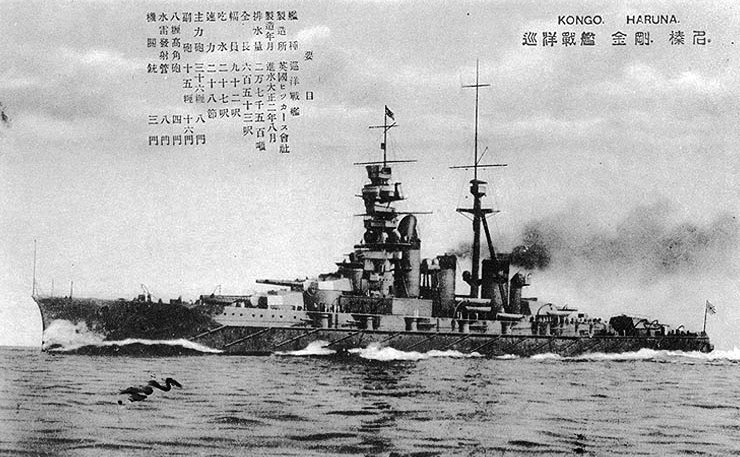
\includegraphics[scale=0.4]{Glava4/x3e2uh2m9tE.jpg}
	%	\label{fig:scipion} % Unique label used for referencing the figure in-text\end{document}
	%	%\addcontentsline{toc}{figure}{Figure \ref{fig:placeholder}} % Uncomment to add the figure to the table of contents%----------------------------------------------------------------------------------------
	\caption{Линейный крейсер Харуна типа Конго в 1925}%	CHAPTER 2
\end{figure}

Три корабля с водоизмещением в 31 700 тонн, каждый из которых был создан от момент закладки и до спуска всего за год - это уже весьма неплохо. Дальше - больше. В марте и ноябре 1912 в Куре и Йокосуке соответственно были заложены Фусо и Ямасиро - вполне современные на дату закладки суда, способные потягаться с любым морским противником со своими 12 356-мм орудиями ГК и вполне приличным бронированием. Затем - небольшая пауза, чтобы позволить кораблестроительной промышленности без задержек довести до ума уже заложенные суда. Причём, важно понимать, что неуклонно улучшались не только количественные, но и качественные показатели. Так, если Квати и Сэтцу были кораблями малоудачными, а серия Конго делалась по английским чертежам и технологиям (а первенец - и вовсе на верфях Альбиона), то уже линкоры Фусо были продуктом чисто японского переосмысления и адаптации проекта Конго, а дальше сложилась своя, сильная и самобытная конструкторская школа. Это при том, что незадолго до начала дредноутной эры, почти все японские броненосцы были куплены за границей.

1915 год стал началом новой крупной линии-генерации, открывшись в мае линкорами Исэ и Хюга. 

\begin{figure}[h!tb] 
	\centering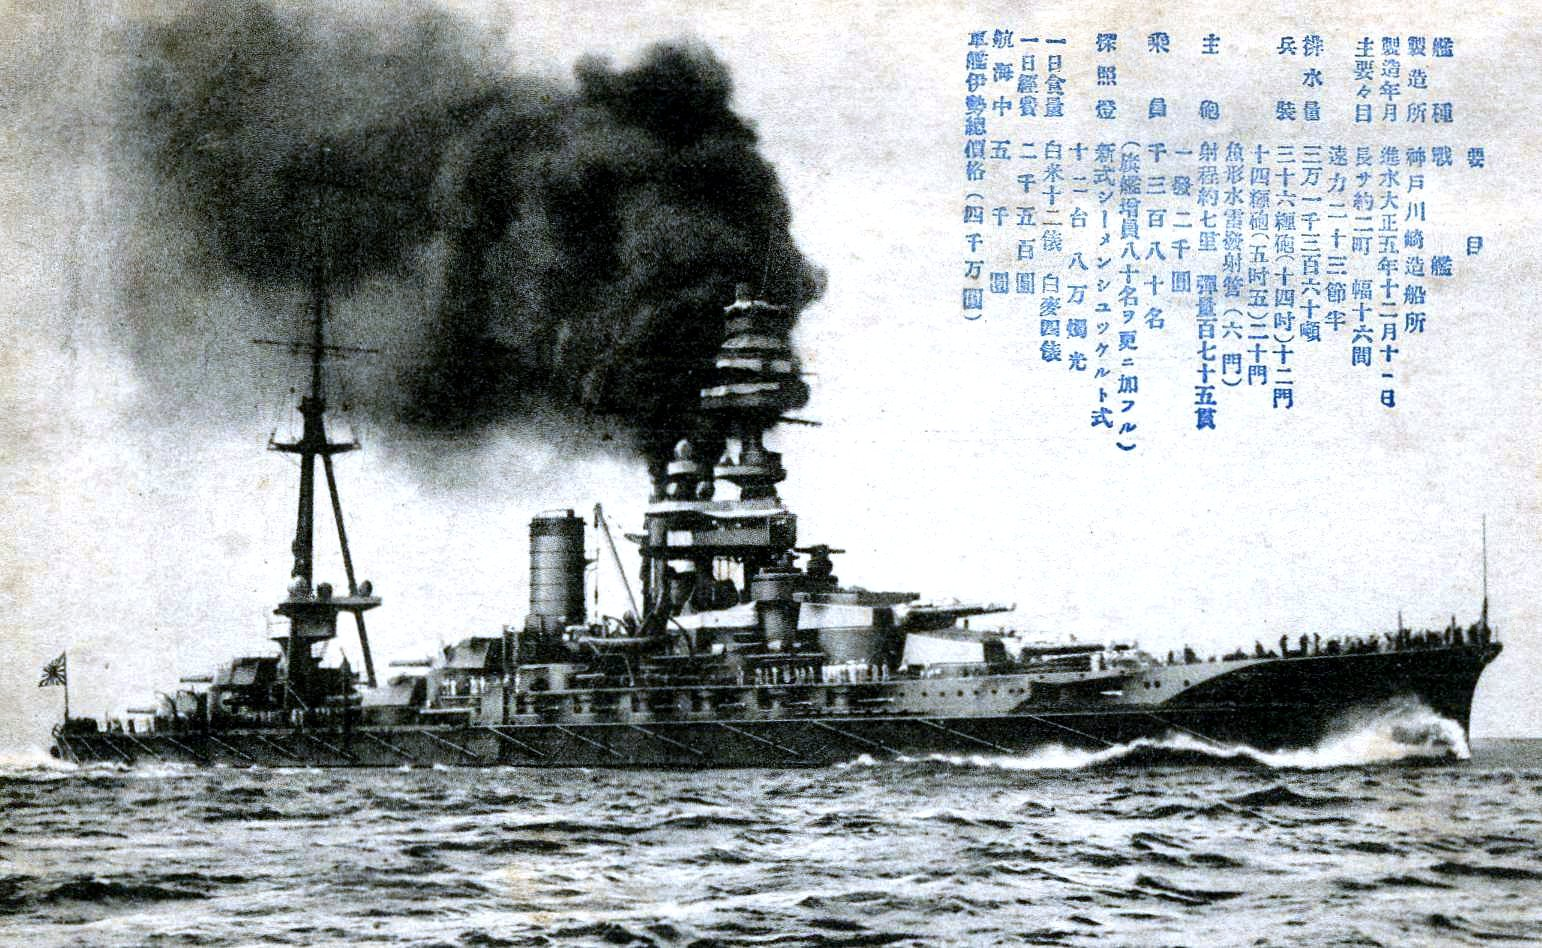
\includegraphics[scale=0.35]{Glava4/_GZCSlPbPmg.jpg}
	%	\label{fig:scipion} % Unique label used for referencing the figure in-text\end{document}
	%	%\addcontentsline{toc}{figure}{Figure \ref{fig:placeholder}} % Uncomment to add the figure to the table of contents%----------------------------------------------------------------------------------------
	\caption{Линейный крейсер Харуна типа Конго в 1925}%	CHAPTER 2
\end{figure}

В 17-м и 18-м годах будут заложены современные, быстрые - скорость до 26,5 узлов, мореходные и вообще весьма сильные близнецы-дредноуты типа Нагато. Их ГК был представлен 8 410-мм пушками (к слову, вплоть до появления японского же Ямато с его 460-мм орудиями, это был самый крупный калибр для морской артиллерии). В 20-м и 21-м годах было заложено сразу 2 линкора и 4 линейных крейсера - об их судьбе мы ещё поговорим подробнее. Только один флот мира в это время усиливался темпами, сравнимыми с японскими - и это флот США.

Именно в это время Соединённые Штаты становятся объектом сравнения, а их морская мощь - поводом для того, чтобы выбивать дополнительное финансирование для военных программ. Планы США стали в обязательном порядке приниматься во внимание. Так, когда в 1916 году Конгресс США одобрил программу строительства для американского флота десяти линкоров и шести линейных крейсеров (в итоге так и не реализованную), в виде ответа на неё 14 июня 1917 года японский парламент утвердил "Комплексную программу флота 8-4" ("Хачи-Си Кантай Кансей Кейкаку"). Программа предусматривала строительство в течение ближайших семи лет трех линкоров и двух линейных крейсеров. Причём командование флота и это посчитало недостаточным и настаивало на увеличении строительства флота, продвигая программу "8 - 8", предусматривавшую создание ударной силы военного флота из 8 линкоров и 8 линейных крейсеров.

При этом нужно сразу сказать, и речи о войне ещё не шло. Вообще американская сила была скорее страшилкой, или, вернее, во вполне японском духе, стыдилкой, фактором в большей мере внутренней политики. Однако, важно отметить вот что: до активизации в Китае, до 21 требования такого рода сопоставления просто никому не приходило в голову тащить за пределы узко военной касты, обсуждать в парламенте, в прессе. Соединённые Штаты начинают восприниматься в качестве страны, которая, косвенными, мирными методами, но с опорой на реальную силу, сдерживает, или может сдерживать развитие Японии, ведь ни для кого не было секретом то, что любые попытки изменить в свою пользу политику "открытых дверей" в Поднебесной, вызывали противодействие США.

Но вернёмся от флотов к дипломатам - самой важной в 21 требовании была их пятая группа. Согласно ей предусматривалось приглашение японцев в качестве советников по политическим, финансовым и военным вопросам при центральном правительстве Китая, признание права земельной собственности в Китае для японских храмов, больниц и школ, создание японо-китайских военных заводов при научно-технической помощи Японии, предоставление Японии прав на строительство железных дорог на китайской территории, консультации с Японией по вопросам строительства железных дорог, рудников и портов в провинции Фуцзянь, предоставление японцам права религиозной пропаганды в Китае.

По сумме 21 требование делало всю громадину Китая, пусть не по названию, но по сути своей протекторатом Японской империи. Только японцы смогли бы извлекать основную коммерческую выгоду из китайского рынка, они получали бы приоритетные права на добычу и продажу китайских природных ресурсов, а главное – сперва негласно, а потом публично направляли бы через институт советников всю политическую и общественную жизнь Поднебесной. Именно советниками именовались английские представители в туземных княжествах и государствах Британской Индии. И японцы готовили Китаю очень похожую судьбу. И ставших локальными царьками и ванами вместо магараджей командиров военных клик тоже встречали бы в Пекине строго нормированным количеством орудийных залпов…

Разумеется, в Китае было немало людей, которые хорошо это понимали – президент-полуимператор Юань Шикай – в их числе, но страна была слишком разобщена и ослаблена, чтобы возможным был общенациональный подъём в борьбе против закабаления. Фактически единственной возможной стратегией для китайцев была затяжка времени, а главное – привлечение за это самое время внимания максимально возможного числа великих держав, которые, естественно, не из альтруистического желания защитить независимый статус Поднебесной, но из нежелания упускать свою выгоду и видеть чересчур усилившуюся Японию в виде конкурента, защитили бы страну от японских притязаний. Проблемой было то, что Первая Мировая была в самом разгаре. Пекин мог быть уверен, что действия Страны Восходящего солнца мало кому понравятся, предполагать, что они встретят дипломатическое осуждение, но лишь надеяться и довольно робко на то, что кто-то сможет реально надавить на Японию достаточно сильно, чтобы она вынуждена была отказаться от своих замыслов. Никто при этом не мог гарантировать, что в случае слишком явного нежелания принимать условия японцев те просто не пойдут от Циндао на север, к столице, по дороге заключив все необходимые договора с каким-нибудь особенно амбициозным генералом, которого и сделают новым главой Китая.

Юань Шикай действовал с традиционной для себя хитростью: с одной стороны он фактически дал добро на четыре первых группы требований, что, в общем, тоже давало Японии большие выгоды и преимущества. С другой – громко, публично, призывая весь мир в свидетели, при том, что японцы предполагали сугубо двусторонний и секретный характер переговоров, отклонил пятую – решающую. Реакция держав могла обнадёжить скорее правительство Страны Восходящего солнца – все были слишком сильно заняты, слишком не хотели получать дополнительного потенциального противника в виде Японии, чтобы реально помогать Китаю. Исходя из этого, пятая группа требований с повестки не снималась. Китайцы тянули время как только могли. В марте 1915 они, наконец, кое-чего дождались: госсекретарь США Уильям Брайан передал 13 марта 1915 года так называемую «ноту Брайана», в которой, признавая «особые интересы» Японии в Маньчжурии, Монголии и Шаньдуне, выражал обеспокоенность ущемлением суверенитета Китая.

На самом деле, конечно, будь Китай образца 1915 нормальным государством, будь он хоть в относительной форме, такого рода ноты должны были бы вызывать закономерное негодование и официальный недвусмысленный и резкий ответ – фактически американцы признавали, что на части территории Поднебесной японцы вправе распоряжаться и хозяйничать, но настоятельно просили не заглатывать всё целиком. Однако, в реальности данный документ был воспринят едва не как спасение. Он придал Юань Шикаю смелости на оставшуюся часть месяца. Ну а дальше началась уже внутренняя политика. Именно в это время Шикай запланировал и начал готовить реставрацию монархии в своём лице – активные мероприятия в этом духе начались с августа месяца. 

\begin{figure}[h!tb] 
	\centering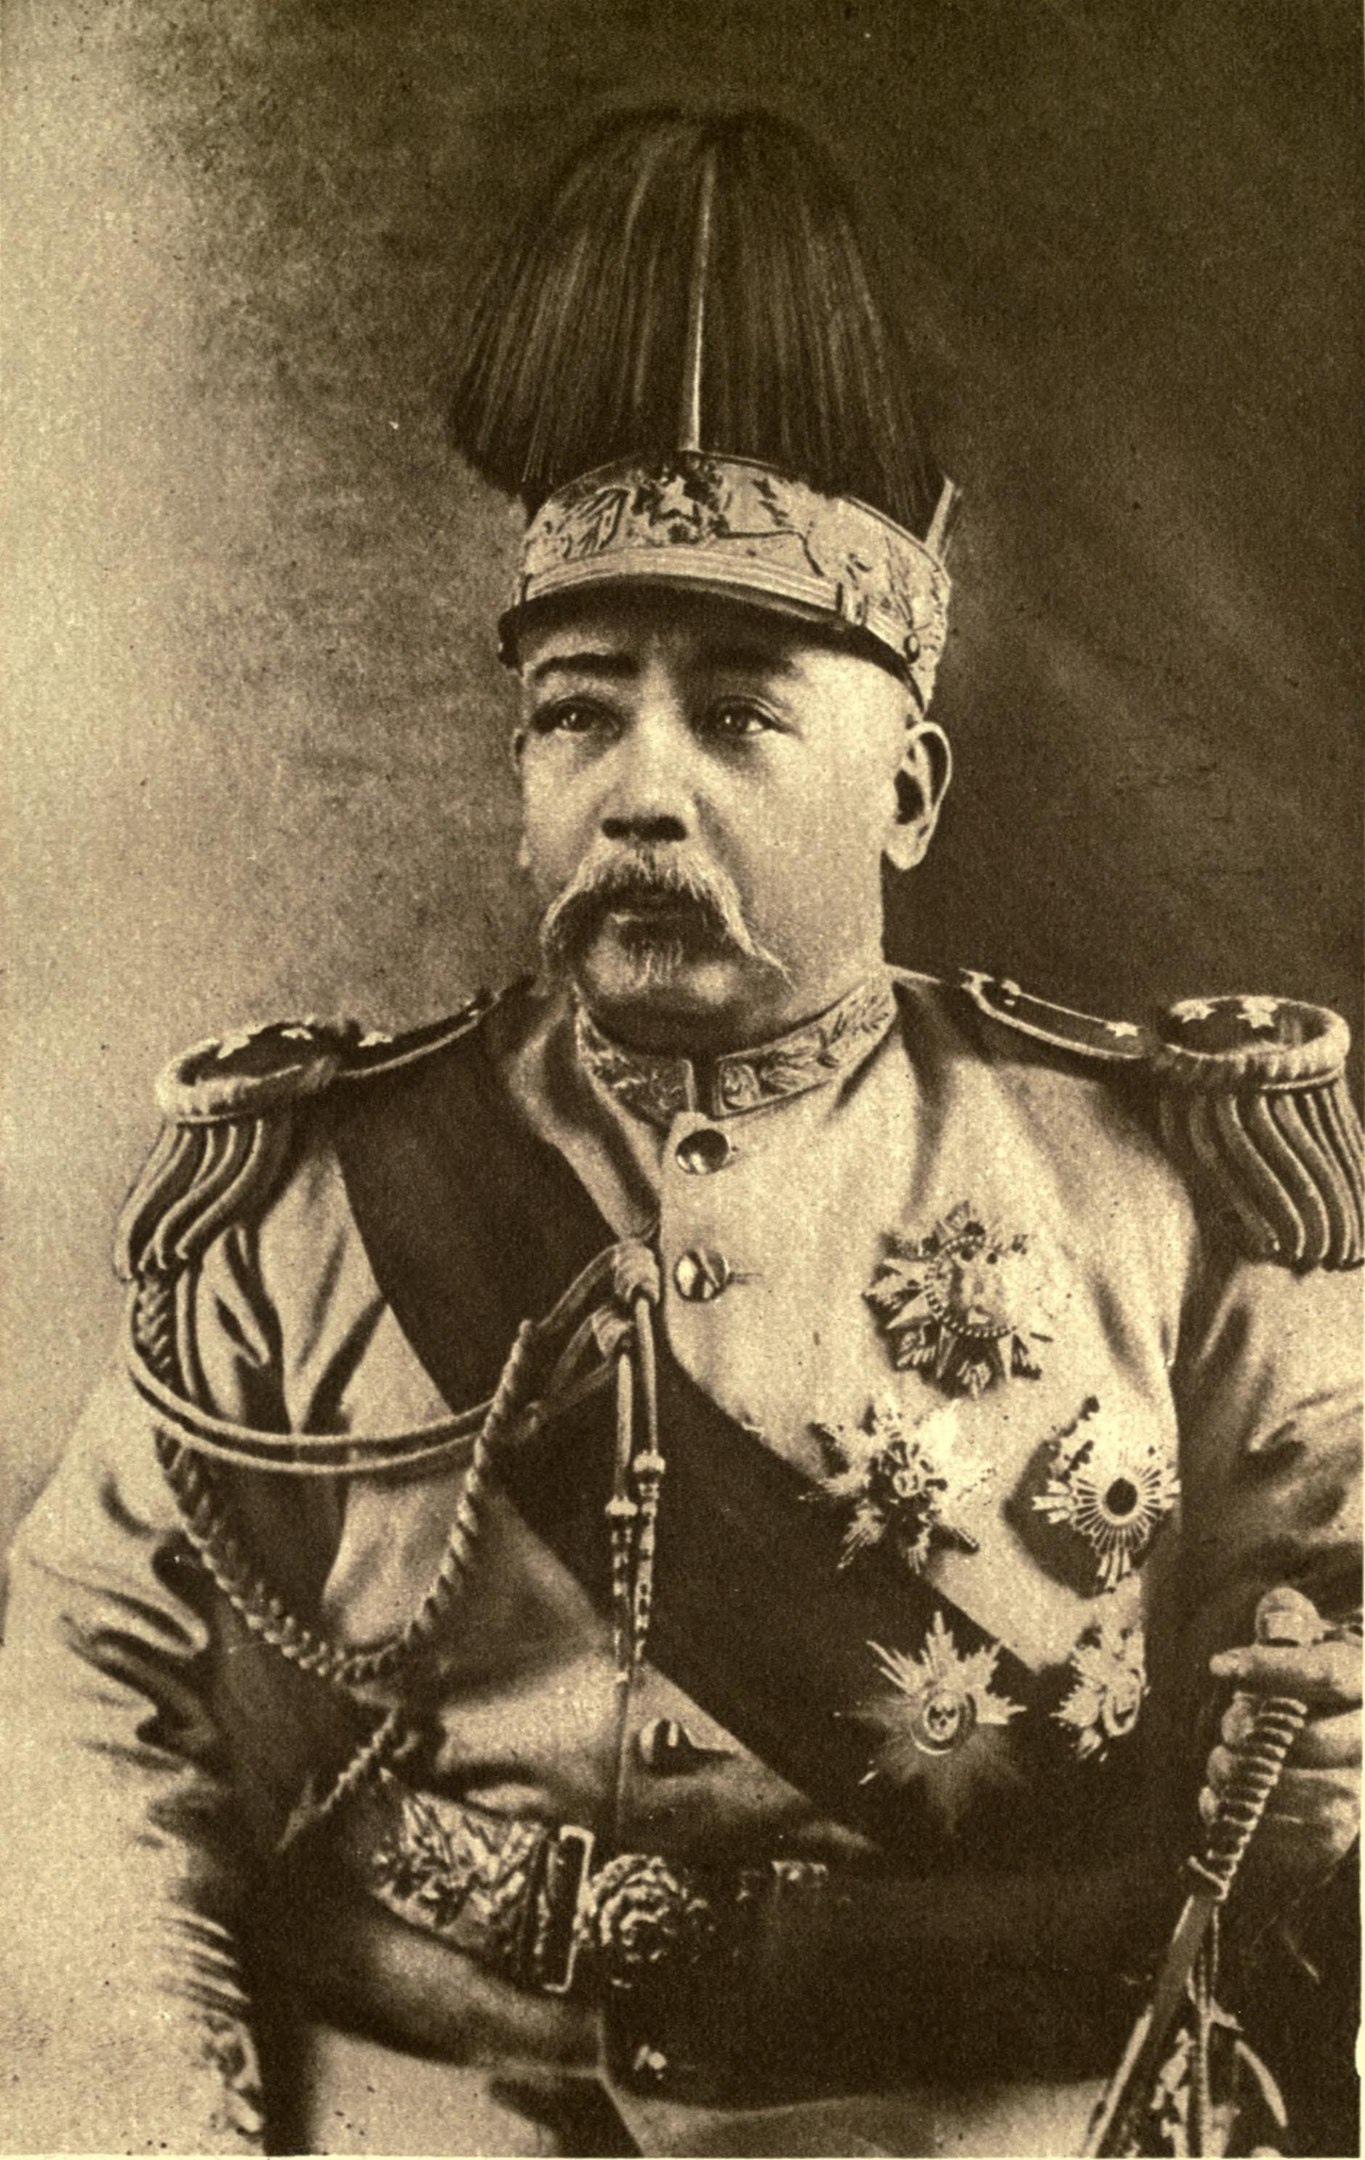
\includegraphics[scale=0.3]{Glava4/ypp_fMADLfk.jpg}
	%	\label{fig:scipion} % Unique label used for referencing the figure in-text\end{document}
	%	%\addcontentsline{toc}{figure}{Figure \ref{fig:placeholder}} % Uncomment to add the figure to the table of contents%----------------------------------------------------------------------------------------
	\caption{Юань Шикай — президент и немножко император Китая}%	CHAPTER 2
\end{figure}

В этих условиях, как ни посмотри, нужно было проявлять твёрдость. Во-первых, принять требования японцев значило сразу и резко подорвать свой авторитет в массах. Новый император мог сделаться популярным, а власть его – прочной только в том случае, если он будет восприниматься (не обязательно быть, но хотя бы восприниматься) сильным, не таким, как свергнутые маньчжуры. 21 требование в полном их виде сделались бы величайшим унижением в истории Китая со времён Опиумных войн – а ведь во многом именно из-за усталости от постоянных унижений вспыхнула Синьхайская революция. Во-вторых, в случае принятия японских условий, реальная власть новоявленного императора оказалась бы более чем ограниченной. А в третьих Юань Шикай держался на вершине в первую очередь за счёт исключительных умений по политическому манёвру (вплоть до степени “вовремя предать означает предвидеть”), а 21 требование слишком жестко завязывало его именно на прояпонские силы и делало врагом для всех тех, кто не желал терпеть вмешательства Японской империи, а таких определённо оказалось бы больше. Наконец, вообще императорский статус в том же году слишком явно смахивал бы на щедрую оплату измены. Юань Шикай не столько из патриотизма, сколько из желания банально не свернуть себе шею, решил отказать Империи Восходящего солнца – впрочем, как всегда, не полностью, оставляя себе лазейки для отступления. 26 апреля 1915 китайцы подтвердили, что твёрдо и безусловно отвергают пятую группу требований. Теперь мяч был на стороне Японии – она могла как счесть это окончательным отказом, так и продолжить переговоры, смягчив условия.

Попутно, очевидно, именно при Юань Шикае китайцы начали продумывать, в общем, довольно детскую, но, как им казалось, спасительную хитрость. Суть её проста: Китай должен был примкнуть к Антанте. Естественно, ни в каких реальных военных действиях армия Поднебесной участвовать не могла, да и не собиралась, благо вероятность появления наземных контингентов Центральных держав в Восточной Азии была строго равна нулю. Но зато китайцы очень хотели оказаться в стане победителей и, пользуясь этим, дезавуировать с опорой на союзников японские притязания. Ведь мы же тоже были с вами в чёрный час опасности и риска! Суровая реальность международной политики была такова, что даже вполне деятельное участие в боях не всегда вело к учёту политических требований и интересов – хорошо прочувствуют это на себе после окончания ПМВ арабы. Но, отложим до поры тему Китай и Антанта, благо в 1915 он к ней и не присоединился, и вернёмся к Японии.

Чтобы понять, кто и как отвечал на действия Юань Шикая, нужно понять как вообще зародился текст документа 21 требования, кто был главным политическим инициатором его появления. И, для начала стоит обратить внимание на саму форму его подачи – бумага была без особенных шума и совершенно без помпы передана японским послом в Пекине. Не министром иностранных дел, не специальным представителем, что соответствовало бы истинной значимости документа. А ещё, что тоже очень важно, император не значился даже формальным автором – 21 требование исходило и пересылалось от имени премьер-министра. С учётом реальной дееспособности (а вернее её отсутствия) Тайсё, заинтересованные лица, написав текст, легко могли опубликовать его как императорский без каких-либо правок и вмешательства с его стороны, если им это было бы нужно. Но нет. Всё вышеописанное суммарно означает одно – 21 требование всё же не было жестким ультиматумом. От слов монарха, особенно широко растиражированных, было бы крайне трудно отказаться даже частично без потери лица. Тихо врученную обычным посланником бумагу за подписью премьера можно было обсуждать. Не было и ясно установленного срока ответа. Правда, опять же, подобная “мягкость”была направлена не столько на китайцев, сколько на внешних игроков. В целом существовало глобально три возможности. Первая – Китай сразу или почти сразу принимает все условия. Естественно, большего японцы и желать не могли. Вторая, реализовавшаяся в действительности – китайцы жестко против какой-то части требований, но готовы идти на компромисс по другим. Она была возможна или если бы Китай сохранил бы переговоры в тайне, или, если их обнародование не вызвало по-настоящему резкой реакции держав. И, наконец, третья – положения 21 требования разглашаются, и за этим следует жесткий и, главное, деятельный ответ тех или иных крупных игроков. Вот тут как раз очень ценным могло оказаться заранее обеспеченное пространство для манёвра.

Надо думать, что наиболее настойчивыми японцы были в конце февраля-начале марта 1915, когда с момент передачи бумаги прошло уже более месяца и не было никаких признаков серьёзных движений со стороны держав. Но, мы помним, 13 марта госсекретарь США Брайан пишет свою ноту. И за китайским отказом 26 апреля теперь уже не гремят сразу пушки...

Изначальным автором 21 пункта, похоже, действительно был премьер-министр Окума Сигэнобу. Профессиональный дипломат (в 1888—1889 годах занимает должность Министра иностранных дел в кабинетах Ито Хиробуми и Курода Киётака, повторно занимал должность Министра иностранных дел, а также ряд других во втором кабинете Мацуката Масаёси в 1896—1897 годах), он, однако, во-первых был уже очень стар при своём 1838 году рождения, а во-вторых в 1907 году как казалось – навсегда, а на самом деле на целых 7 лет, уходил их политики. 

\begin{figure}[h!tb] 
	\centering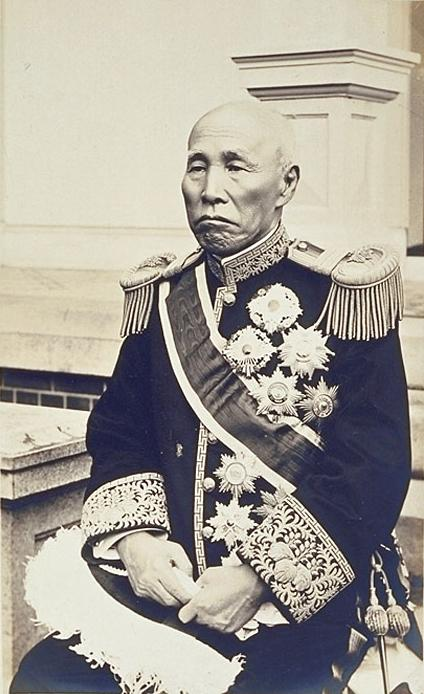
\includegraphics[scale=0.4]{Glava4/-n7yRkLYs2g.jpg}
	%	\label{fig:scipion} % Unique label used for referencing the figure in-text\end{document}
	%	%\addcontentsline{toc}{figure}{Figure \ref{fig:placeholder}} % Uncomment to add the figure to the table of contents%----------------------------------------------------------------------------------------
	\caption{Окума Сигэнобу}%	CHAPTER 2
\end{figure}

Не вызывает сомнений, что 21 требование, получившее, в числе прочего, скажем, официальное одобрение парламента, проверялось и визировалось в первую очередь Гэнро. Они же принимали окончательное решение о войне, мире или компромиссе в конце апреля 1915. Итоговый вариант имел классический для дипломатии вид уменьшения требований с одновременным их ужесточением. Пятая группа – наиболее принципиальная, чреватая для Китая постепенным превращением в колонию, была удалена, но оставшиеся 4 были вновь переданы Юань Шикаю уже в виде ультиматума 7 мая 1915. Срок ответа – 2 дня. Юань Шикай никак не мог пойти на риск войны с Японией, и вообще ему лично куда как более импонировала стратегия «умиротворения». Империя Восходящего солнца получила утвердительный ответ. Договор был подписан 25 мая.

Победа? Определённо. Но не без горького привкуса. И дело не просто в том, что первоначальный список требований был принят не полностью. Наиболее серьёзным было то, что нынешний успех, тем не менее, порождал весьма неопределённое будущее. Да, чрезвычайно ослабленный внутренне Китай в весьма специфических условиях, когда международное положение оставляло его практически один на один с Японией, был вынужден пойти на обширные уступки. Но всё это вполне могло со временем перемениться. Юань Шикай – дополнительно укрепить свою власть, страны Антанты, завершив с успехом войну, или США, довооружившись и проведя соответствующую подготовительную кампанию в обществе, могли вмешаться, требуя пересмотра договорённостей 1915. Империя Восходящего солнца приобрела многое, но не приобрела главного: фактического контроля над системой власти Поднебесной, либо, что тоже её устроило бы, не смогла поставить под сомнение её суверенность и субъектность. Царьков Британской Индии никто не считал субъектами международной политики – это просто была такая форма управления британскими, по сути, территориями. В Китае японцы хотели добиться того же – но не смогли. И теперь угроза отмены или ревизии принятых 13 требований висела дамокловым мечом, заставляя Японию всё активнее вооружаться, дабы никто не рискнул пытаться прогнуть её силой. В частности США. Особенно США. И за ними нужно пристально следить. Не давать им слишком сильно превзойти Японию в области морских вооружений (про дредноутные программы японцев уже было сказано выше). Вот – самый первый симптом того, что в будущем станет жестоким антагонизмом.

Однако пока, повторюсь, это победа. В августе 1915 года премьер-министр Сигэнобу провёл реорганизацию своего правительства и помимо должности премьера занял должность министра иностранных дел – судя по всему действия министра иностранных дел в период, так сказать, острой фазы переговорного процесса с китайцами – Като Такааки были оценены неудовлетворительно. Впрочем, может быть, дело и не в этом – в ходе выборов в парламент марта 1915 всплыло на поверхность и разгорелось несколько коррупционных скандалов, а тесная связь Такааки с дзайбацу Мицубиси была общеизвестной, так что ему нужно было уйти. Это отнюдь не стало концом его политической карьеры – в 1924-1926 он даже сам сделается премьер-министром. Но вернёмся к Сигэнобу. Очевидно, именно его посчитали тем, кто в первую очередь обеспечил успешное принятие большей части требований – и соответствующим образом отметили. В июне 1916 года за заслуги перед державой император наградил его титулом косяку (условный японский аналог маркиза, нередко так и переводится). Правда, уже в октябре того же года кабинет Сигэнобу в полном составе ушёл в отставку, но, вероятно, ключевой причиной тут был возраст, а не политика. Во всяком случае, оставшуюся жизнь он прожил в большом почёте, а в похоронной церемонии в парке Хибия после смерти Сигэнобу 10 января 1922 года, приняли участие десятки тысяч людей.

Япония могло оплакивать смерть своего государственного мужа, но куда важнее для неё объективно была другая кончина. 6 июня 1916, почти тогда же, когда Окума Сигэнобу стал маркизом, в Китае скончался от уремии Юань Шикай. Ему было всего 56, так что, конечно, все ожидали более долгого его правления. А главное… Генерал, премьер-министр в период империи, первый президент республики, без пяти минут новый император, Юань Шикай был большим мерзавцем. Он плёл интриги, он обманывал, он плевать хотел на народ, его чаяния и его тяготы он был тщеславным, он был жестоким, но он мог держать Поднебесную в узде. Его власть в общекитайском хаосе была чуть ли ни единственной прочной вещью. Его не назовёшь “успешным менеджером”, не назовёшь лидером нации, не назовёшь вождём – он не решил ни одной из глобальных задач, стоявших перед Китаем, и очень мало кто искренне любил его – та же история с референдумом об императорской власти – чистой воды постановка, где режиссёрами были местные чиновники и офицеры. Но Юань Шикай не давал стране вовсе расползтись. С его смертью же Китая практически не стало. Остались клики, группы военных и гражданских руководителей (в первую очередь, конечно, генералов), объединённых исключительно личными связями, а ещё чаще – землячеством, а не какими бы то ни было идеями, сражающиеся за власть, не чураясь никакими способами, потому что победа противной стороны с большой долей вероятности означала смерть. Власть в Пекине становилась с каждым годом, да даже месяцем всё более номинальной. В стране разгоралась гражданская война, причём по худшему сценарию – не условные “красные против белых” а провинция против провинции.

Непосредственно после смерти президента, его прерогативы перешли к вице-президенту с 1912 по 1916 год, позднее избравшемуся на высший пост – Ли Юаньхуну. 

\begin{figure}[h!tb] 
	\centering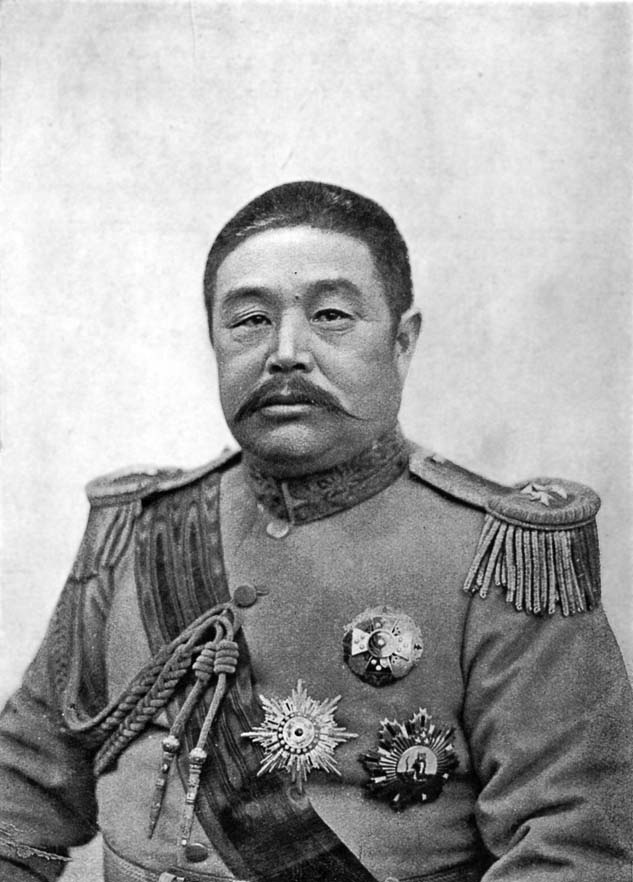
\includegraphics[scale=0.8]{Glava4/PQ6zgwNhs98.jpg}
	%	\label{fig:scipion} % Unique label used for referencing the figure in-text\end{document}
	%	%\addcontentsline{toc}{figure}{Figure \ref{fig:placeholder}} % Uncomment to add the figure to the table of contents%----------------------------------------------------------------------------------------
	\caption{Ли Юаньхун}%	CHAPTER 2
\end{figure}
Ещё один военный, он, тем не менее, был человеком не слишком решительным – вероятно Юань Шикай приблизил его к вершине именно потому, что знал – тот не рискнёт пытаться столкнуть оттуда его самого. Истинные правители позволили ему стать номинально главным по двум причинам. Первая – чтобы у народа был объект для критики и “спуска пара” не затрагивающий их интересов. Вторая – чтобы конкурирующие клики не имели формального повода для обвинений в узурпации. Кем же были эти реальные властители? Так называемая Аньхойская клика получила своё название от провинции Аньхой, уроженцами которой были лидеры клики Дуань Цижуй и другие. 

\begin{figure}[h!tb] 
	\centering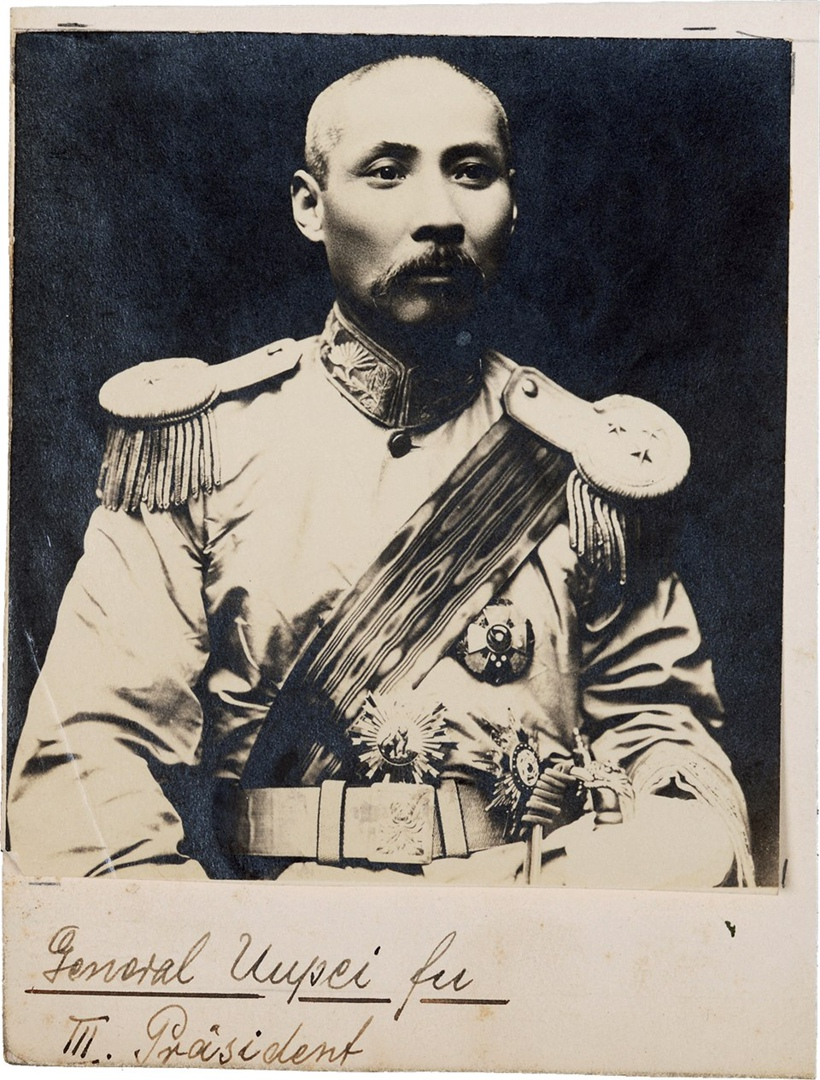
\includegraphics[scale=0.4]{Glava4/WVQAAPD5EGk.jpg}
	%	\label{fig:scipion} % Unique label used for referencing the figure in-text\end{document}
	%	%\addcontentsline{toc}{figure}{Figure \ref{fig:placeholder}} % Uncomment to add the figure to the table of contents%----------------------------------------------------------------------------------------
	\caption{Дуань Цижуй}%	CHAPTER 2
\end{figure}

Вообще, как уже было сказано, ключевым признаком и принципом было землячество. Предпосылки для формирования клики как фракции в Бэйяньской армии были заложены ещё в самом конце XIX века могущественным сановником Ли Хунчжаном, который тоже происходил из Аньхоя. Военные силы клики размещались в провинциях Хэнань, Чахар, Чжили, Шаньдун и во Внешней Монголии. Эти силы и использовались кликой для утверждения своего господства в Северном Китае. Вообще именно силовая, если не сказать вооружённая составляющая была основой власти клики, которая была ничем иным, как замаскированной военной диктатурой. Дуань Цижуй, бывший ещё с 1896 подчинённым и близким соратником Юань Шикая, с 1912 года занимал пост военного министра. В 1916 он сделался премьером, довольно быстро оттеснив после этого президента от рычагов управления. Власть Цижуя была даже более твёрдой, жестокой и автократической, нежели у Шикая, но, и это принципиально важно, только на части территории страны – той, которая твёрдо контролировалась войсками Аньхойцев. Там, а также вблизи Пекина, слово премьера было законом. В зоне же влияния других клик, при формальном признании власти президента и премьера (прежде всего для того, чтобы не ставить под сомнение территориальную целостность Китая, чем мгновенно могли бы воспользоваться те же японцы, да и не только они) на большую часть распоряжений Цижуя плевать хотели. 

\begin{figure}[h!tb] 
	\centering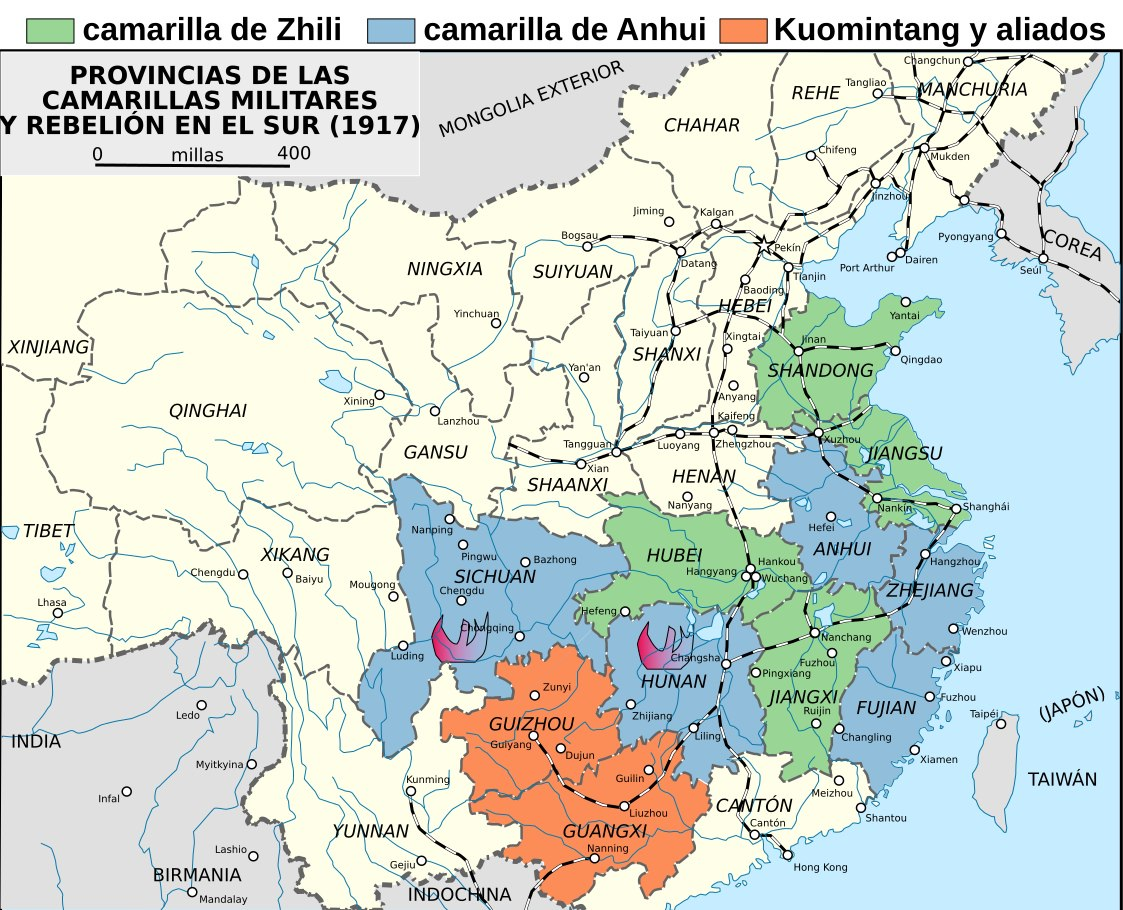
\includegraphics[scale=0.4]{Glava4/Z1CcQ3h0vFA.jpg}
	%	\label{fig:scipion} % Unique label used for referencing the figure in-text\end{document}
	%	%\addcontentsline{toc}{figure}{Figure \ref{fig:placeholder}} % Uncomment to add the figure to the table of contents%----------------------------------------------------------------------------------------
	\caption{Китай, разделённый между кликами, на 1917 год}%	CHAPTER 2
\end{figure}

Всё это ставило Японию в довольно специфическое положение. Правительства, которое могло бы гарантировать исполнение условий 13 требований на всей территории Поднебесной, просто не существовало. Аньхойская клика, как самая сильная, стала получать определённую поддержку от японцев, но это мигом сделало её врагами все остальные клики. Естественно, они не желали знать, что там подписывалось и кем ещё при Шикае, если им это не было выгодно. А если таким образом можно ещё и японцам насолить, то просто замечательно. Япония в первый раз столкнулась с дилеммой, которая ещё аукнется ей не раз позднее: чтобы контролировать Китай, нужно, чтобы там было сильное правительство, которое могло бы заставить региональные элиты уважать и соблюдать межгосударственные договорённости, но, стоило этой сильной власти стать чуть могущественнее определённого предела, как уже она сама начинала ставить под сомнение и ревизовать навязанные японцами в момент слабости документы. Тот же Дуань Цижуй с удовольствим брал японские деньги, использовал их ресурсы, но отнюдь не был “прояпонским” политиком и где конспиративно, а где и открыто наступал им на ноги, если это могло ему что-то дать, или он рассчитывал их обмануть. Японцы всё понимали, видели, но терпели, ибо альтернатива – совсем уже полный хаос в Китае, который придётся разгребать вооружённой рукой – а это означает война не с центральным правительством, которое можно заставить делать всё что угодно после взятия Пекина, а со всеми провинциями разом. И нужен тут не 30-40 тысячный экспедиционный корпус, который стоял в Циндао, а огромная армия в полмиллиона, а лучше – больше. В 1910-х Япония была не готова сделать такой выбор. Во второй половине 1930-х ситуация изменится…

А пока Цижуй с одной стороны пытался удержать и упрочить власть, а с другой после паузы, попытался всё же реализовать комбинацию, задуманную ещё Шикаем – Китай в Антанте. Это могло как позволить Поднебесной после завершения войны попытаться отменить договор о 13 требованиях, так и в ходе неё выпрашивать у той же Японии и других стран-противников Германии кредиты и оружие. Но неожиданно глава кабинета министров натолкнулся на довольно активное противостояние президента. Сложно сказать, чего именно боялся Ли Юаньхун. К началу 1917 года и дураку было ясно, что Центральные державы находятся в тяжёлом положении, а уж Китаю просто никак не могут угрожать. Вероятно, основной страх был опять таким связан с внутренней политикой: народу нужно было хоть как то объяснить, почему страна вступает в совершенно чужую для неё войну – и всякие такие объяснение могли нарушить довольно хрупкий порядок, при котором низовые, простонародные массы удавалось удерживать от колоссальных масштабов бунта. Поди докажи крестьянину или даже горожанину, что война – это лишь формальность, а местные власти не станут по этому поводу драть с него три шкуры!

В конечном итоге объявление войны Германии и Австро-Венгрии стало возможным только после падения президента. Оно же в свою очередь произошло по причине монархического путча июля 1917. Началось всё с того, что в мае 1917 президент при помощи парламента отправил лидера Аньхойской клики в отставку с поста премьера. Скорее всего, Юаньхун не рассчитывал на то, что Дуан Цижуя удастся, в самом деле, выкинуть из политики – скорее всего президент наивно рассчитывал вернуть генерала на его пост по достижению некоего компромисса. Вот только Аньхойской клике компромиссы были не нужны. По требованию Цижуя верные ему местные военные губернаторы объявили, что они не подчиняются больше Пекину и потребовали у Ли Юаньхуна сложения с себя полномочий президента. Причём подразумевалось, что в случае отказа данная операция будет произведена насильственно, вооруженной рукой. Президент срочно стал искать, на кого он мог бы опереться. Другим кликам Юаньхун был не особенно нужен – у них были свои кандидаты, так что в итоге был найден высокий чином, но второразрядный с точки зрения реальной власти генерал по имени Чжан Сюнь. Никто и подумать не мог, что уже довольно немолодой и давно никак себя не проявлявший Сюнь поведёт свою игру. Вероятно, определённую роль здесь сыграло немецкое посольство, в котором знали, что в самом скором времени после победы Аньхойцев, Китай вступит в войну. Реально дипломаты Кайзеррейха мало чем могли помочь Чжан Сюню, но вот воодушевить, заставить играть честолюбие… Утром 1 июля 1917 году Чжан Сюнь вошел с войсками в Пекин и… неожиданно для всех объявил о реставрации Цинской монархии, вернул на трон Пу И и тоже потребовал у Ли Юаньхуна сложения полномочий, на что тот сразу ответил отказом. Впрочем, на президента всем уже было наплевать – началась другая игра. В поднебесной после Синьхайской революции царил такой чудовищный и всё нарастающий хаос, что народу идея реставрации вполне могла прийтись по вкусу. Что ещё хуже, она могла прийтись по вкусу японцам. Так что у Аньхойской клики времени на то, чтобы реализовать своё военное преимущество, было в обрез. Дуань Цижуй самым быстрым темпом повёл свои войска на Пекин. Чжан Сюнь заперся в Запретном городе. Начались бои. 

\begin{figure}[h!tb] 
	\centering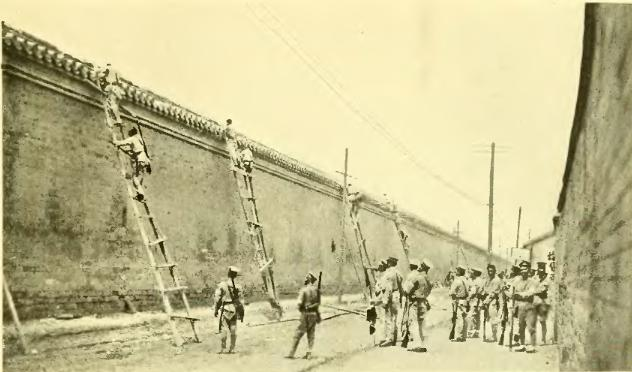
\includegraphics[scale=0.6]{Glava4/yj5aMs32FGM.jpg}
	%	\label{fig:scipion} % Unique label used for referencing the figure in-text\end{document}
	%	%\addcontentsline{toc}{figure}{Figure \ref{fig:placeholder}} % Uncomment to add the figure to the table of contents%----------------------------------------------------------------------------------------
	\caption{Штурм Запретного города}%	CHAPTER 2
\end{figure}

Один из самолётов Дуаня даже бомбил Запретный город, что, возможно, стало первой бомбардировкой в Восточной Азии. К 12 июля побеждённые войска Чжана разбежались, и Дуань вернулся в Пекин. Занятно, что сам заговорщик смог избежать смерти, или даже просто какого-либо наказания, так как укрылся в голландском посольстве, где и попросил политического убежища. Больше Чжан Сюнь участия в политике не принимал.

Тем временем в течение беспорядков вице-президент Фэн Гочжан, ещё один бывший бэйянский генерал, занял пост исполняющего обязанности президента и принял присягу в Нанкине. Дуань Цижуй вновь получил пост премьер-министра. Ли Юаньхуна выбросили, как старое тряпьё, 17 июля 1917 без какого-либо противодействия с его стороны или со стороны кого-то ещё. Затем Дуань Цижуй разогнал парламент, осмелившийся его снять по указанию уже бывшего президента. А 14 августа 1917 Китай объявил войну Германии и Австро-Венгрии, став, тем самым, формальным союзником Японии – к немалой досаде последней. Война же, тем временем, затягивалась, и всё сильнее проявлялись её глобальные экономические последствия. Одним из таких был достаточно существенный рост цен на продовольствие в мировом масштабе. Кушать, как известно, надо всем – в том числе и многомиллионным армиям, выпавшим из процесса производства. Не менее важным был и распад существовавших хозяйственных связей, блокады, угроза транспорту, особенно морскому, заставлявшему судовладельцев и фрахтовщиков включать риски в стоимость. Зима 1916-1917 года здесь стала рубежной для многих стран. В Германии она известна как Брюквеная. В одном из самых, если не самом развитом государстве планеты, несмотря на достаточно хорошо отлаженную систему карточного распределения, начался натуральный голод. Суммарно от голода и недоедания во Втором Рейхе за 1914-1918 умерло около 800 000 человек, из них подавляющее большинство – именно в Брюквеную зиму. В Российской империи нехватка хлеба в столице, послужившая поводом к началу Февральской революции, была вызвана скорее отвратительной логистикой (а частично, вероятно, и саботажем), но и с продовольствием ситуация ухудшалась буквально на глазах, чтобы стать по-настоящему тяжёлой уже во второй половине 1917 года. Даже контролирующая моря и имеющая массу незатронутых или слабо затронутых войной колоний Британская империя была вынуждена ввести ограничения на свободную продажу продовольствия в конце 1917.

Япония же уже к началу войны априори зависела от ввоза продуктов – так же, как и Альбион, вот только у Империи Восходящего солнца колоний не было, только Корея, которая не могла дать много, без риска того, что голод начнётся уже в ней. Последствия и угрозы были достаточно очевидны – тем не менее, японское правительство умудрилось не предпринять никаких значимых мер до того, как кризис оказался на пороге. Возможно, свою роль сыграло то, что, собственно, количественной нехватки не было почти до самого конца – условные прилавки не были пусты, но вот цены выросли и весьма существенно. Высшие классы могли почувствовать некоторый дискомфорт, но не более того, в то время как для основной части японцев нищета стала или реальностью, или, как минимум, весьма грозным и близким призраком.

Руководители же Японии чересчур заигрались в большую международную политику. При этом всё больше становилась диспропорция между тем, что государство могло рассчитывать получить в перспективе в результате своих дипломатических побед, и тем, чем можно воспользоваться прямо сейчас. Теоретически, пусть даже и принятое в неполном виде, 21 требование давало японцам решающее преимущество в Китае по сравнению со всеми другими игроками, а это могло принести громадные дивиденды. Но прямо сейчас, в 1916, 1917, 1918 годах это не давало решительно ничего! Поднебесная была настолько раздроблена и слаба, что туда по-прежнему было и опасно вкладываться, и сама её экономическая жизнь из-за непрерывного внутреннего конфликта, всё чаще – вооружённого, заметно сдала. Напротив, пока выходило, что Япония должна спонсировать не особенно-то дружественную и “свою” Аньхойскую клику, а главное, в расчёте на будущую оборону от притязаний других держав – политическо-договорную, или реальную, того, что она успела получить в Китае, пока они были заняты, усиливать свои вооружённые силы. Особенно флот. Дредноуты Япония научилась строить и качественно, и быстро, но менее дорогими они от этого не становились. Такими же темпами флот, как было сказано выше, рос только в США, но при этом благосостояние Америки, величина её промышленности, финансового сектора, покупательная способность населения были несопоставимы с японскими. Иными словами, при тех же номинальных величинах, доля в государственных тратах выходила совершенно иной. Штаты могли себе позволить новые дредноуты без особенного напряжения. Японцы – если ещё не переставляя дырки на ремне, то, по крайней мере, не оставляя свободных резервов на другие проекты и цели. Стране нужен был умный и расчётливый хозяйственник, который смог бы, во-первых, не упустить из виду возможность социального взрыва, а во-вторых весьма точно свести дебет с кредитом либо сократив часть расходов, либо изыскав дополнительные источники дохода.

Вместо этого на пост премьер-министра, ставший весьма важным в отсутствии дееспособного императора и постепенном ослаблении (в силу вымирания) института Гэнро, после отставки Сигэнобу был назначен Тэраути Масатакэ, человек, котором стоит сказать подробнее. 

\begin{figure}[h!tb] 
	\centering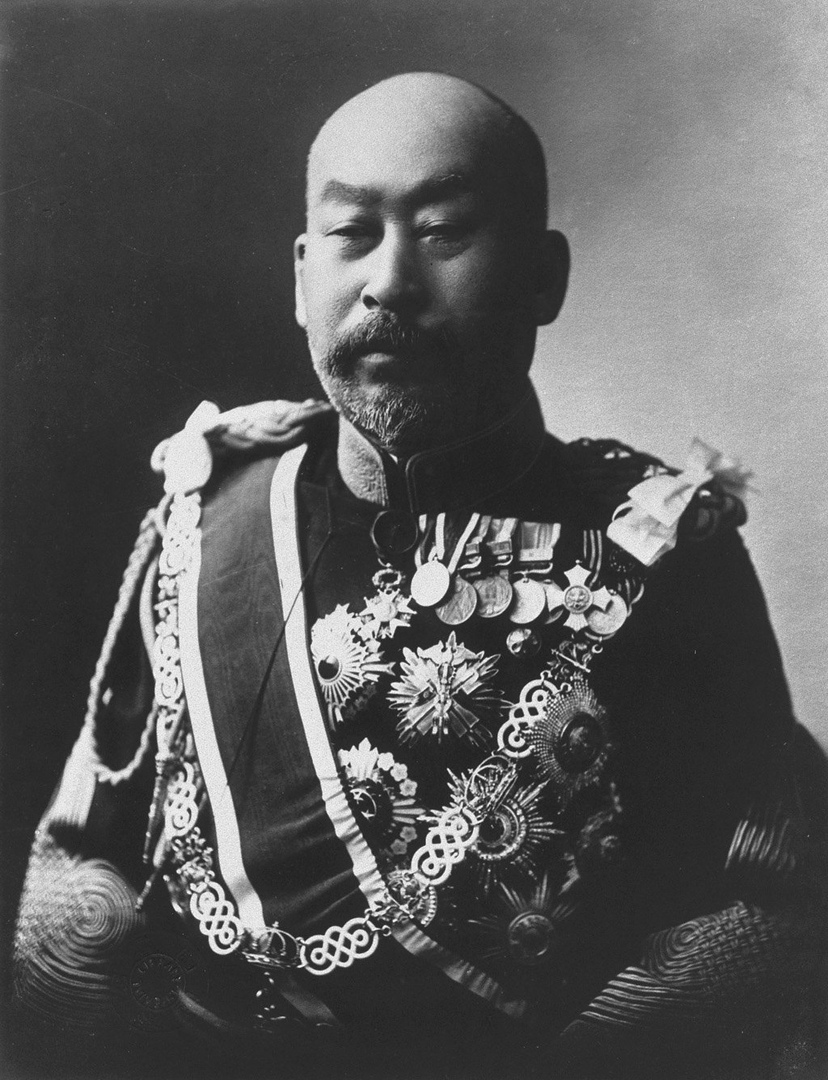
\includegraphics[scale=0.4]{Glava4/cjLahz3MIWA.jpg}
	%	\label{fig:scipion} % Unique label used for referencing the figure in-text\end{document}
	%	%\addcontentsline{toc}{figure}{Figure \ref{fig:placeholder}} % Uncomment to add the figure to the table of contents%----------------------------------------------------------------------------------------
	\caption{Тэраути Масатакэ}%	CHAPTER 2
\end{figure}

В первую очередь нужно отметить, что это – военный. Да, в Японии Мэйдзи нередко бывало, что талантливые представители высшей элиты одновременно имели высокие посты по гражданской и высокие звания по военной линии. Но Масатакэ был чистым офицером, многие годы отдавшим службе, потерявшем ещё в 1877 году в ходе подавления восстания самураев в Сацуме руку, который от начала карьеры и до 1910 года вообще службы, не связанной напрямую с военным делом, не исправлял. В 1882 году Тэраути Масатакэ был военным атташе во Франции. После этого, в 1898 году, он был назначен первым главным инспектором боевой подготовки. В 1901 году он стал министром армии в первом кабинете Кацуры Таро. Он оставался в должности и в течение Русско-японской войны, что, естественно, после победного её окончания, резко повысило его престиж и вес. После войны ему были последовательно присвоены титулы барона, а в 1911 году — графа. И вот, наконец, в 1910 гражданский пост – генерал-резидент в Корее. Вот только направлялся туда Масатакэ как чистый силовик, если не каратель, призванный установить жесткий и надёжный контроль над страной Утренней свежести. Причиной было убийство борцом за независимость и корейским националистом Аном Чунгыном пожалуй самого выдающегося из деятелей эпохи Мэйдзи, первого из Гэнро, упоминавшегося в предыдущих частях Ито Хиробуми 26 октября 1909 года. Дело было так:

В октябре 1909 года Ито Хиробуми выехал в Харбин для встречи с российским министром финансов В. Н. Коковцовым. Планировалось обсудить вопрос о полной аннексии Кореи Японией. 26 октября в 9 часов утра поезд, на котором ехал Ито, прибыл на станцию. 

\begin{figure}[h!tb] 
	\centering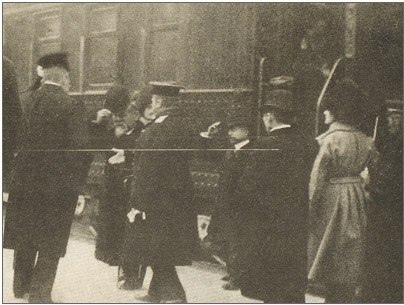
\includegraphics[scale=0.6]{Glava4/VU6yNahIz7w.jpg}
	%	\label{fig:scipion} % Unique label used for referencing the figure in-text\end{document}
	%	%\addcontentsline{toc}{figure}{Figure \ref{fig:placeholder}} % Uncomment to add the figure to the table of contents%----------------------------------------------------------------------------------------
	\caption{Оригинальное фото, сделанное за несколько минут до убийства}%	CHAPTER 2
\end{figure}

После того, как Коковцов зашёл в вагон, Ито тепло поприветствовал его и высказал уверенность, что между Японией и Россией всегда будут мир и дружба. Коковцов предложил ему сойти на платформу, где выстроился почётный караул. Когда они совершали обход караула, Ито Хиробуми был застрелен корейским националистом Ан Чунгыном. Он умер через полчаса после покушения. Последними словами Ито были «Он застрелил меня. Вот дурак!».

Многоопытный гэнро был прав – Чунгын действительно совершил глупость: если покойный выступал за достаточно мягкий, поэтапный процесс включения Кореи в состав Империи Восходящего солнца, то после его убийства дело очень ускорилось, ужесточилось, а несогласные стали подвергаться откровенным репрессиям. Итак, после небольшого, полугодового промежуточного периода, когда обязанности генерал-резидента Кореи исполнял Сонэ Арасукэ, чей послужной список был составлен из мирных, гражданских занятий хозяйственного толка: он был министром юстиции в третьем кабинете Ито Хиробуми, министром сельского хозяйства и коммерции во втором кабинете Ямагаты Аритомо и министром финансов в первом кабинете Кацуры Таро (1901—1906), на его место приходит Масатакэ. Он прибыл в Корею 30 мая 1910 – и в кратчайший срок сперва составил, а потом продавил Договор о присоединении Кореи к Японии. Происходило всё скорее как военная операция, нежели дипломатическая договорённость. Подписанный 22 августа 1910 документ открывался словами «Его Величество Император Кореи полностью и бессрочно передает Его Величеству Императору Японии все суверенные права на управление Кореей» – больше похоже на капитуляцию. И сам Масатаэ смотрел на дело так же. Не чуждый поэзии, он сочинил по случаю успеха хокку: “Что бы подумали Кобаякава, Като и Кониси, если бы жили они сейчас, взглянув на луну сегодня вечером?”, где Кобаякава, Като и Кониси – генералы армии сёгуна Тоётоми Хидэёси, воевавшие в Корее и пытавшиеся её захватить в 1592-1598.

Затем уже в качестве не генерал-резидента, а генерал-губернатора Кореи, Тэраути Масаткэ провёл ряд весьма непопулярных мер и реформ, в частности начал процесс японизации - по его приказу в Корее было открыто несколько тысяч школ, где изучался японский язык и японская литература. Также Тэраути провёл земельную реформу в Корее: был создан земельный кадастр, однако составлялся он исключительно на основе письменных документов, между тем как земельные отношения в Корее зачастую регулировались с помощью обычного права. Это привело к утрате земли значительной частью корейских крестьян. Земля перешла в государственный фонд, что облегчало размещение на ней японских переселенцев. Все выступления, начиная от самых первых – против Договора и потери даже фиктивной независимости, подавлялись военными средствами. И вот именно этот человек, окончательно подчинив и замирив Корею, 9 октября 1916 становится премьером Японии. Вскоре после этого он получает звание маршала. Почему, зачем был сделан именно этот выбор? Судя по дальнейшим его действиям, Масатакэ должен был резко интенсифицировать силовое давление на Китай. В идеале оно должно было завершиться таким же, как в Корее, проталкиванием в режиме блиц устраивающего Японию документа – возможно отвергнутой китайцами части 21 требования.

Масатакэ развивает кипучую деятельность. Он даже добивается неформального понимания от США, которые вновь признали «особые интересы Японии в Китае». Штаты как раз вступили в войну, и теперь тоже не могут себе позволить активно лезть в дела Китая. Также маршал-премьер серьёзно нарастил степень влияния на Аньхойцев и вообще достиг ситуации, когда без японцев ни один значимый вопрос в Китае объективно не решался – пока ещё не в том смысле, что им всегда шли на уступки, но в том, что их стало совершенно невозможно игнорировать. Даже в случае с Монголией и Тибетом и их спорах с Пекином японцы играли важную роль. Сложно сказать, успел бы Масатаке дожать Китай, или нет. Мне представляется, что всё же нет. Но тут вмешался непредвиденный фактор – революция в России. Фактор, который заставит разгореться японские амбиции, и, погнавшись за двумя зайцами, потерять время. А его даже не внешние игроки, а сам японский народ, исстрадавшийся из-за дороговизны, отвёл уже не так много.

Об участии Японии в Интервенции, последствиях этого участия, а главное – о Рисовых бунтах и итогах политики Империи Восходящего солнца в Китае и её участия в Первой мировой войне – в следующей части.

\url{https://vk.com/wall-162479647_83282}